% TODO textcommand für Scenegraph-Ebene, SimpleMesh-Ebene, Icon-Ebene

\newpage
\section{Umsetzung}
Im Folgenden wird das Mockup, die Implementierung, sowie die Evaluierung des Prototyps beschrieben. Bei der Skizzierung der Mockups und auch während der Implementierung wurde auf eine gute Benutzerfreundlichkeit geachtet. Hierfür wurde sich an den 1994 von Nielsen entwickelten 10 Usability Entscheidungsregeln \cite{Nielsen.1994} orientiert. Im kommenden Kapitel \ref{sec:UsabilityHeuristics} wird genauer geprüft wie gut diese eingehalten wurden.

\subsection{Mockup}\label{sec:Mockup}
Für den Prototyp wurden Mockups skizziert an dessen Aufbau und Design sich während der Implementierung orientiert wurde. Diese Mockups wurden zunächst auf Papier niedergeschrieben und für die folgende Beschreibung mithilfe von Figma \cite{Figma} digitalisiert. Es gibt jeweils ein Mockup für die Übersicht, Steuerung und Verwaltung, sowie für das Routenplanungs-Popup.

Abbildung \ref{fig:MockupOverview} im Anhang zeigt das Mockup für die Übersicht. In der Übersicht werden die Raummodelle zusammen mit den verschiedenen Roboterdaten angezeigt. So werden die Standorte mithilfe von Icons, die Roboterpfade mithilfe von Linien und die Roboterpositionen mithilfe von 3D-Modellen der Roboter dargestellt. Es gibt außerdem Buttons mit denen zwischen den verschiedenen Stockwerken navigiert werden kann und mit denen die Roboter ausgewählt werden können. Zusätzlich gibt es einen Button, der es ermöglicht den ausgewählten Roboter automatisch zu verfolgen und einen anderen Button mit dem die Kameraposition wieder zur Ausgangsposition zurückgesetzt werden kann. Die Buttons sind abhängig von ihren Funktionen in den vier Ecken der Anwendung gruppiert.

Die Steuerung in Abbildung \ref{fig:MockupControls} im Anhang erweitert die Übersicht um weitere Funktionen und sieht daher fast identisch zur Übersicht aus. Der einzige Unterschied sind zusätzliche Buttons mit denen eine Lieferroute bestimmt, der Roboter zum Aufladen geschickt, oder der aktuelle Lieferauftrag abgebrochen werden kann. Die Abbildung \ref{fig:MockupRoutePlanner} im Anhang zeigt das Mockup für das Routenplanungs-Popup das sich öffnet, wenn der Lieferroute-Button ausgewählt wird. In dem Popup muss ein Ziel und ein Roboter ausgewählt werden, bevor der Auftrag gestartet werden kann. 
% TODO zusätzliche Funktionen erwähnen? => Auch können optional ein Ausgabepunkt und Zwischenstationen eingestellt werden.
Um die Routenerstellung zu vereinfachen, sollen sowohl Roboter als auch Standorte zusätzlich über das Anklicken auf der Karte auswählbar sein.

Die Abbildung \ref{fig:MockupAdministration} zeigt das Mockup für die Verwaltung. Hier gibt es jeweils eine Liste für die Roboter und die Stockwerke. In der Liste der Roboter können verschiedene Informationen der einzelnen Roboter, wie beispielsweise der systeminterne \ac{ID} und die Neustartzeit ausgelesen werden. Auch können Einstellungen der Roboter, wie Name und Ausgabepunkt geändert werden. Zudem gibt es für jeden Roboter eine Vorschau der Übersicht, in der die Position des Roboters gezeigt wird. Sowohl in der Liste der Roboter als auch in der Liste der Stockwerke gibt es für jedes Stockwerk eine Auflistung der Standorte. In der Liste der Stockwerke gibt es außerdem eine Vorschau der Übersicht und zusätzlich ein Kontextmenü, über das in den Editiermodus des Stockwerks gewechselt werden kann. In diesem sollen die Roboterdaten und Stockwerke manuell synchronisiert werden können. Für den Editiermodus wurde kein Mockup entworfen, da das Aussehen zu stark von den Möglichkeiten in \deckgl{} abhängt, die noch nicht vollständig bekannt waren, als die Mockups entworfen wurden und erst während der Implementierung bekannt wurden. Aus diesem Grund wurde bestimmt, dass das Aussehen des Editiermodus während der Implementierung festgelegt werden muss.

\subsection{Implementierung}
Es wurde ein Frontend entwickelt, dass auf das \ac{BCB} zugreift, um die Roboterdaten anzufragen. Wie das \ac{BCB} hierbei mit den Robotern kommuniziert, wird im Kapitel \ref{sec:BotControlBackend} erklärt. Das Frontend nutzt das Web-Framework React in Kombination mit \ac{HTML}, \ac{SCSS} und Typescript. Die Vorteile von Typescript und \ac{SCSS} gegenüber Javascript und \ac{CSS}, wie auch Web-Framework React wird im Kapitel \ref{sec:WebTechnologies} erläutert.
% Typscript wurde aufgrund der statischen Typisierung, frühzeitigen Fehlererkennung und besseren Wartbarkeit gegenüber Javascript. Da SCSS eine bessere Übersichtlichkeit der Stylesheets ermöglicht, wurde es statt CSS eingesetzt.
Zustandsinformationen die Komponentenübergreifend abgerufen werden, werden zentral mithilfe von React-Redux gespeichert. Die Grundstruktur des Frontend-Projekts wurde mihilfe des Shell Befehls npx create-chayns-app \cite{CreateChaynsApp} generiert. Die Kompilierung ist mithile des \ac{npm}-Pakets chayns-toolkit \cite{ChaynsToolkit} konfiguriert. \ac{GUI}-Elemente wie Buttons und Aufklapper werden durch die Komponentenbibliothek chayns-components \cite{ChaynsComponents} bereitgestellt. Außerdem werden die \ac{npm}-Pakete clsx \cite{clsx} und fortawesome \cite{fontawesome} eingesetzt. Mithilfe von clsx lassen sich HTML Klassennamen Kompackt unter Bedingungen anwenden. Das fortawesome \ac{npm}-Paket wird genutzt, um \ac{SVG} Icons als Zeichenkette zu importieren. Ein großer Teil der Typescript Type-Definitionen konnte aus einem anderen Frontend-Projekt kopiert werden. Hierbei handelt es sich um Types für Objekte, die aus dem \ac{BCB} stammen.

\subsubsection{Übersicht}
In der Übersicht werden die Roboterdaten in Kombination mit den Gebäudemodellen mithilfe von \deckgl{} angezeigt. Hierfür werden verschiedene \deckgl{}-Layers eingesetzt.

\paragraph{Gebäudemodelle}
Für den Prototyp sind die \ac{URL}-Verweise der 3D-Modelle hartkodiert, also in den Quelltext der Webanwendung eingebettet. Für ein potenzielles Produktivsystem müssten die \ac{URL}-Verweise in der Datenbank des \ac{BCB}s abgespeichert werden. Die Modelle sind im chanys.space gespeichert und werden aus Gründen, die in Kapitel \ref{sec:ModelFileFormat} bereits erläutert wurden, im \ac{glTF}-Format geladen und in der ScenegraphLayer angezeigt. Diese Ebene ist dafür ausgelegt, ein bestimmtes 3D-Modell beliebig oft an verschiedenen Positionen anzuzeigen \cite{DeckglScenegraphLayer}, was auf die Hauptfunktion von \deckgl{} - die Visualisierung riesiger Geodaten Mengen \cite{Deckgl} - zurückzuführen ist. Aus diesem Grund muss für jedes 3D-Modell eine eigene Instanz der ScenegraphLayer erzeugt werden. \deckgl{} ist für den Einsatz von über 100 Ebenen gleichzeitig ausgelegt, wobei wahrscheinlich sogar der einsatz von bis zu 1000 Ebenen ohne große Performance Einbußen möglich ist \cite{DeckglPerformance}. Im Prototyp besteht ein Stockwerk aus bis zu sechs 3D-Modellen und somit auch aus sechs ScenegraphLayers. Da nicht davon auszugehen ist, dass jemals mehr als 15-mal so viele Modelle für ein Stockwerk nötig sind, sind keine negativen Performance-Auswirkungen durch den Einsatz einer Ebene für ein einzelnes Modell zu erwarten.
% TODO Zahl anpassen, falls mehr Modelle genutzt werden
Für die Scenegraph-Layers ist das Backface Culling aktiviert. Mithilfe vom Backface Culling werden die von der Kamera weggerichteten Polygone ausgeblendet \cite{BackfaceCulling}. Meist wird Backface Culling genutzt, um Polygone auszublenden, die sowieso hinter anderen Polygonen versteckt sind, um die Darstellungsgeschwindigkeit zu erhöhen. Im Fall der Gebäudemodelle sind die Polygone in den Raum hineingerichtet. Somit bewirkt das Backface Culling, dass die Wände und Decken ausgeblendet werden, die dem Nutzer die Sicht in den Raum verdecken würden. In der Abbildung \ref{fig:BackfaceCulling} wird dieser Effekt verdeutlicht. So sieht man auf der linken Seite, dass ohne das Backface Culling nicht in den Raum hineingesehen werden kann, während es auf der rechten Seite mit Backface Culling möglich ist.

\begin{figure}[H]
    \caption{Raummodell ohne und mit Backface Culling}\label{fig:BackfaceCulling}
    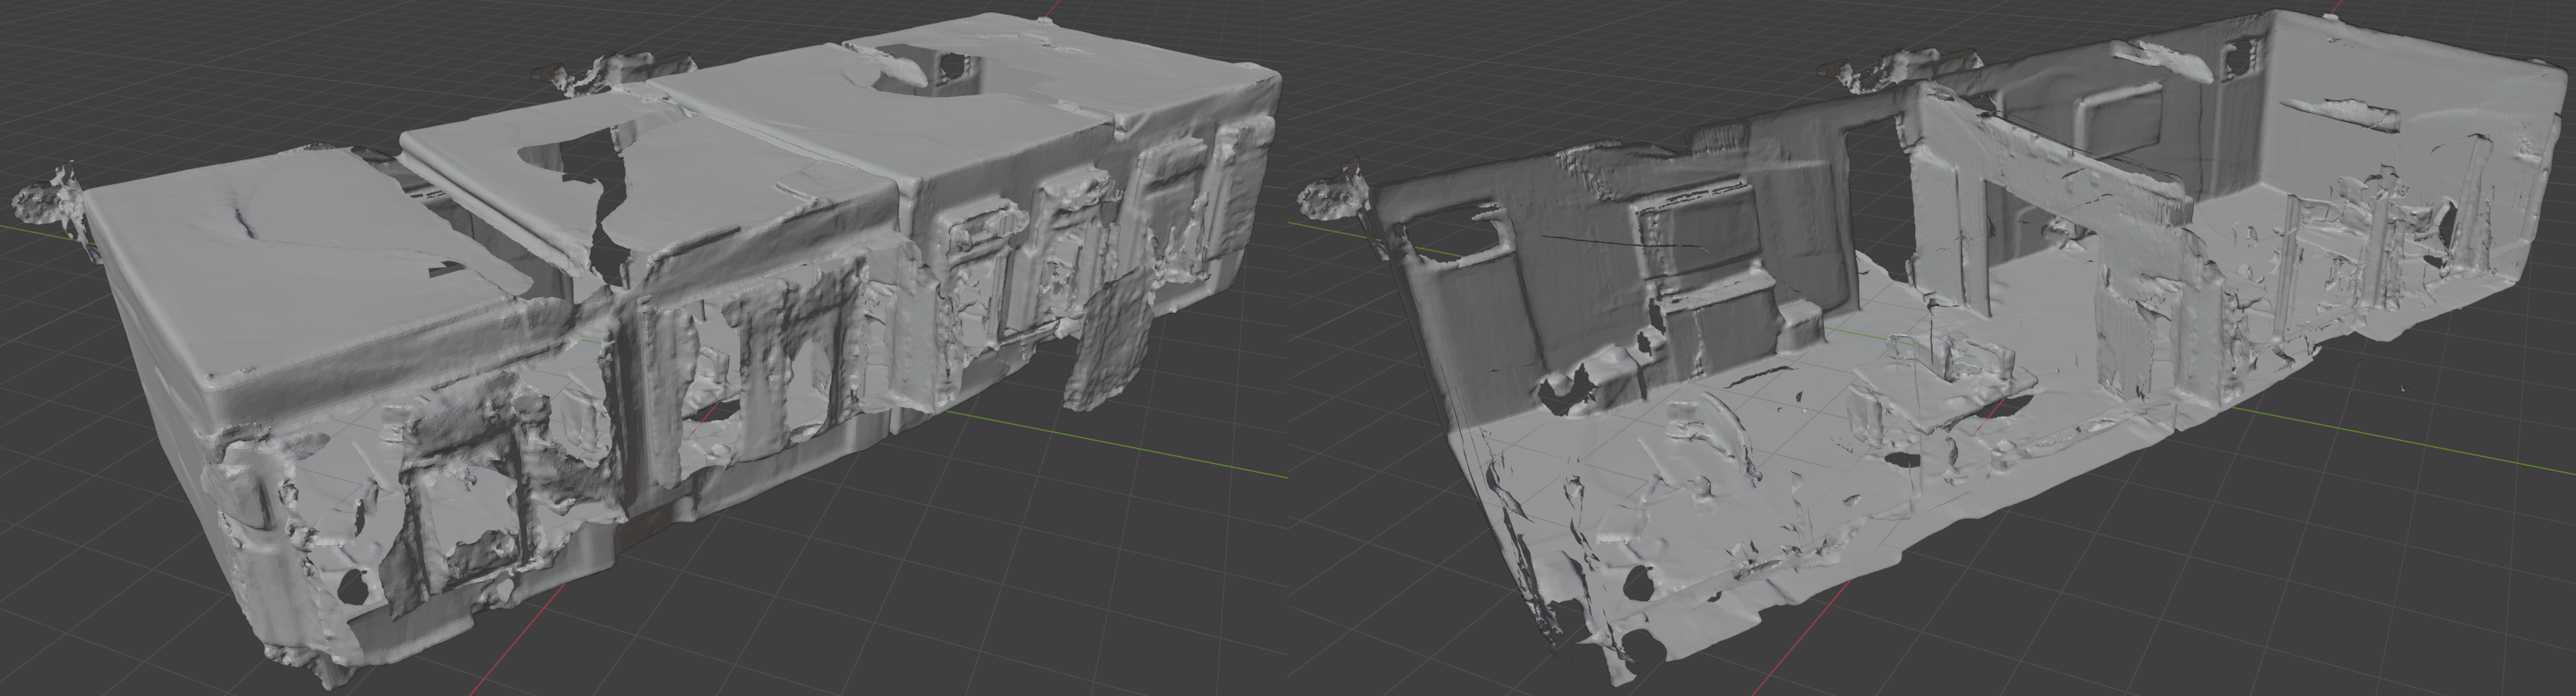
\includegraphics[width=0.9\textwidth]{Backface Culling Vergleich.png}
    \\
    Quelle: Eigene Darstellung
\end{figure}
% TODO Ist "Quelle: Eigene Darstellung" richtig?
% TODO Erwähnen falls 3D-Modelle gecached werden

\paragraph{Roboterdaten}\label{sec:RobotData}
Die Roboterdaten werden über verschiedene Endpunkte des \ac{BCB}s abgerufen. So gibt es einen Endpunkt für die Bezeichnungen der verschiedenen Standorte und einen Endpunkt für den Roboterstatus, Lieferautrag und die Roboterposition \cite{BCBSwagger}. Für die Positionen aller Standorte und der Roboterpfade gibt es keinen Endpunkt. Stattdessen können die Standorte und Pfade nur von Stockwerken angefragt werden, in denen sich Roboter zu dem Zeitpunkt befinden, da diese Daten direkt von den Robotern angefragt werden. Damit immer alle Daten aus allen Stockwerken abgerufen werden können, sind diese Daten im Prototyp für alle Stockwerke hartkodiert. Für ein potenzielles Produktivsystem müssten diese Daten in der Datenbank des \ac{BCB}s gespeichert und regelmäßig mit den Robotern synchronisiert werden.
% Braucht es ein Schaubild in dem die erweiterte Datenbankstrukur dargestellt wird?

Im Gegensatz zu den Gebäuademodellen werden die Robotermodelle im \ac{OBJ}-Format mit der SimpleMeshLayer \cite{DeckglSimpleMeshLayer} angezeigt. Mit der ScenegraphLayer gibt es das Problem, dass die Positionen der Modelle nicht animiert werden können, wodurch die SimpleMeshLayer brauchbarer, aber auch nicht ideal, ist. Laut der Dokumentation voj \deckgl{} sollte das Animieren über die transition Property in allen Ebenen möglich sein \cite{DeckglLayerClass}. Deshalb handelt es sich bei dem Problem mit der ScenegraphLayer vermutlich um einen Bug in \deckgl{}. Wie im Kapitel \ref{sec:ModelFileFormat} erwähnt, lässt sich die Materialdatei des \ac{OBJ} Formats nicht in der SimpleMeshLayer einbinden, weshalb die Roboter einfarbig angezeigt werden müssen. Das ist nicht unbedingt ein Nachteil, denn so können die Roboter mithilfe einer herausstechenden Farbe für den Nutzer besser sichtbar gemacht werden. Die Positionsänderungen der Roboter werden über die transitions Property animiert. Allerdings lässt sich die Rotation nicht animieren, was vermutlich auch auf einen Bug in \deckgl{} zurückzuführen ist.

Über den Robotermodellen wird mithilfe der IconLayer der aktuelle Status der Roboter angezeigt. Während in einer ScenehraphLayer-Instanz nur ein bestimmtes 3D-Modell angezeigt werden kann, können in einer IconLayer-Instanz verschiedene Bilder mithilfe der getIcon Zugriffsfunktion angezeigt werden \cite{DeckglIconLayer}, weshalb hierfür im Gegensatz zur ScenegraphLayer eine Layer-Instanz ausreicht. Die genutzten Icons stammen aus der Icon-Bibliothek Fontawesome und werden aus dem fortawesome \ac{npm}-Paket als \ac{SVG}-Zeichenkette importiert. Da die IconLayer das \ac{SVG} Format nicht unterstützt, werden die \ac{SVG}-Zeichenketten in das Data-\ac{URL} Format umgewandelt. Das Data-\ac{URL} Format bettet Daten als \gls{Base64}-Zeichenkette innerhalb einer \ac{URL} ein \cite{DataUrl}.

Die verschiedenen Standorte werden über die IconLayer angezeigt. Wie bei den Roboter-Zuständen werden hierfür verschiedene Fontawesome-Icons genutzt. Wurde ein Roboter ausgewählt und hat dieser einen Lieferauftrag, dann wird der Zielstandort farbig markiert. Die Pfade und virtuellen Wände werden über eine Instanz der PathLayer \cite{DeckglPathLayer} dargestellt. Die virtuellen Wände werden gestrichelt und in einer anderen Farbe angezeigt, um diese von den Roboterpfaden zu unterscheiden. Für die gestrichelte Darstellung wird die PathStyleExtension \cite{DeckglPathStyleExtension} genutzt.

Bei der Abbildung \ref{fig:OverviewScreenshot} handelt es sich um einen Screenshot der Übersicht im Prototyp. Man sieht alle erwähnten Ebenen, sowie die verschiedenen Buttons. Basierend auf dem Feedback aus den Usability Tests, die im Kapitel \ref{sec:UsabilityTests} genauer beschrieben werden, wurden Buttons ergänzt, die es nicht im Mockup gibt.

\begin{figure}[H]
    \caption{Übersicht}\label{fig:OverviewScreenshot}
    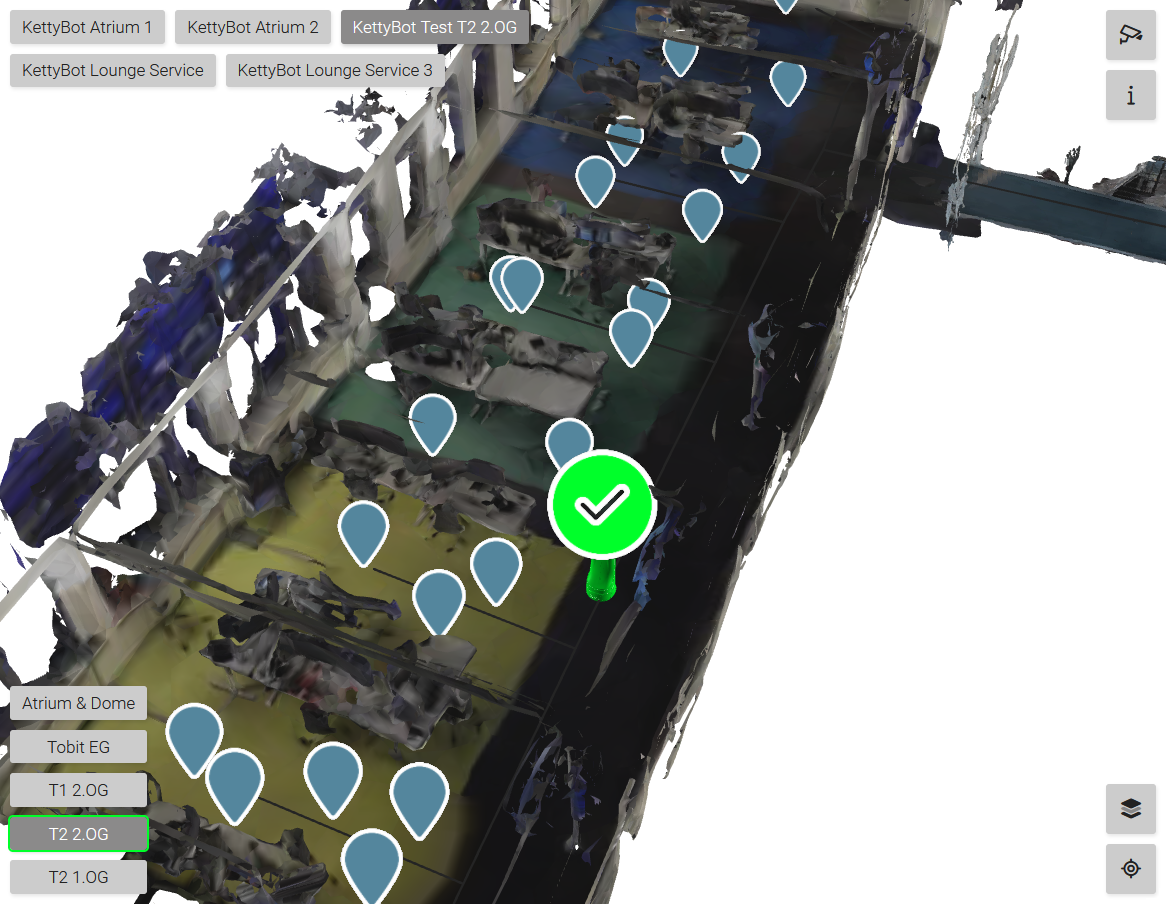
\includegraphics[width=0.9\textwidth]{Screenshot Uebersicht.png}
    \\
    Quelle: Eigene Darstellung
\end{figure}

\paragraph{Echtzeit-Aktualisierung}
Die Positionen sowie weitere Statusinformationen der Roboter, wie beispielsweise der aktuelle Auftrag und Akkuladung, werden mithilfe einer indirekten Verbindung zwischen der Webanwendung und dem \ac{BCB} regelmäßig aktualisiert. Hierfür wird der im Kapitel \ref{sec:Chayns} beschriebene \gls{Websocket}-Service genutzt. In der Abbildung \ref{fig:RobotStatusUpdate} ist der Ablauf einer Statusaktualisierung vereinfacht dargestellt. Aktualisiert ein Roboter seine Position, wird die entsprechende Information über \gls{MQTT} an das \ac{BCB} gesendet. Wie die Kommunikation zwischen Robotern und \ac{BCB} genau funktioniert wird im Kapitel \ref{sec:BotControlBackend} genauer erklärt.
% Passt das so? Funktioniert MQTT wie beschrieben?
Das \ac{BCB} sendet daraufhin eine Nachricht an den \gls{Websocket}-Service, der diese Information wiederum an alle verbundenen Clients schickt, die Nachrichten von dem \ac{BCB} erwarten. So sieht man in der Abbildung auch, dass der dritte Client keine Nachricht empfängt, da dieser Nachrichten von einem anderen System erwartet.

\begin{figure}[H]
    \centering
    \caption[]{Kommunikationsweg von Statusaktualisierungen der Roboter}\label{fig:RobotStatusUpdate}
    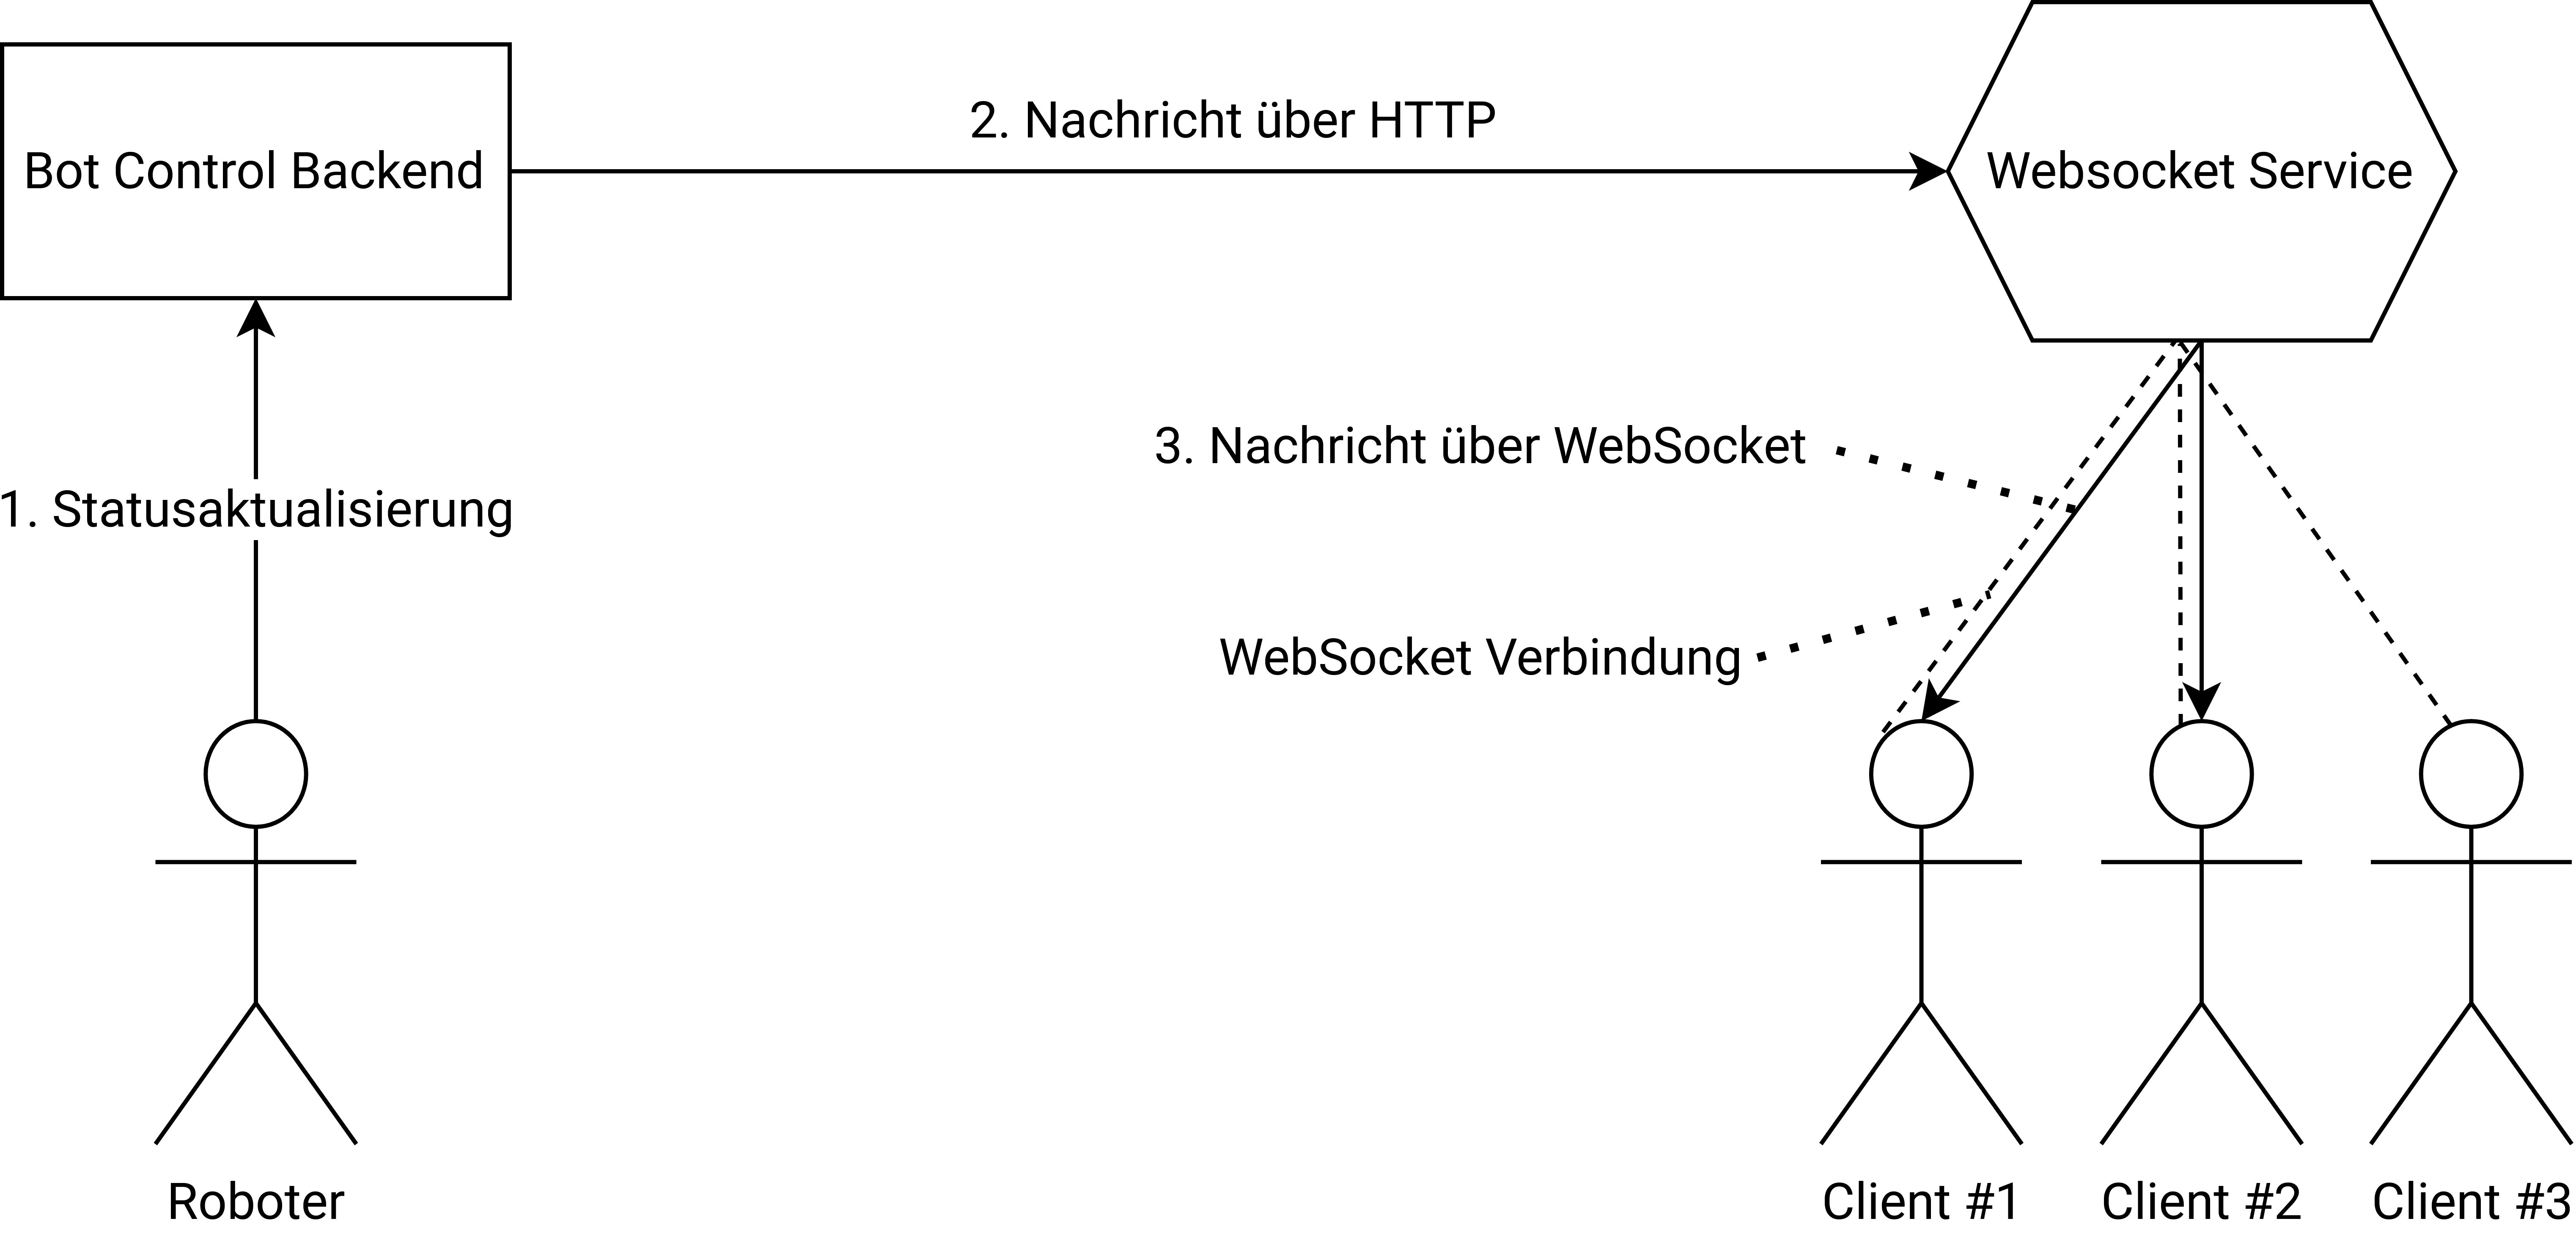
\includegraphics[width=0.9\textwidth]{Websocket Service.png}
    \\
    Quelle: Eigene Darstellung
\end{figure}

Die über den \gls{Websocket}-Service empfangene Statusaktualisierung wird zentral im Redux-Store aktualisiert, sodass dem Nutzer die Aktualisierung direkt angezeigt werden kann. Bei Positonsänderungen der Roboter werden diese mithilfe des transitions Attributs der SimpleMeshLayer und der IconLayer animiert \cite{DeckglLayerClass}. So entsteht der Eindruck, dass die Roboter fahren. Wie im Kapitel \ref{sec:RobotData} erwähnt, lässt sich für die Robotermodelle allerdings nur die Position und nicht die Rotation animieren.

\paragraph{Interaktion}
Die Roboter, sowie die Standorte sind, mithilfe der onClick Property der entsprechenden Ebene \cite{DeckglInteractivity}, auswählbar. Ausgewählte Standorte und Roboter werden verfärbt angezeigt. Außerdem erscheint ein Button über den sich weitere Informationen wie beispielsweise die Akkuladung bei Robotern und der Name bei Standorten anzeigen lässt. Schwebt die Maus über einem Standort oder Roboter, dann wird mithilfe der getTooltip Property \cite{DeckglDeckClass} ein Tooltip angezeigt, in dem der Name des entsprechenen Objekts und weitere wichtige Informationen stehen. Es gibt zudem die Möglichkeit einem Roboter zu Folgen. Die Kamera wird hierfür mithilfe des FlyToInterpolators \cite{DeckglFlyToInterpolator} zu dem ausgewählten Roboter bewegt. Während einem Roboter gefolgt wird, wird die Kameraposition mithilfe der transitionDuration Property \cite{DeckglAnimationsAndTransitions} animiert, wenn die Roboterposition aktualisiert wird.

\subsubsection{Steuerung}
Wie im Kapitel \ref{sec:Mockup} beschrieben, gibt es drei Aktionen die zum Steuern der Roboter mithilfe von Buttons ausgeführt werden können: Lieferauftrag, Laden und Abbrechen. Mit dem Laden und Abbrechen wird der aktuelle Lieferauftrag abgebrochen, worauf der Nutzer auch über einen Bestätigungsdialog hingewiesen wird. Für das Starten eines Lieferauftrags muss ein Ziel und ein Roboter angegeben werden. Hierfür gibt es Inputs, mit denen nach Standorten und Robotern gesucht werden kann. Bei den Inputs handelt es sich um die PersonFinder-Komponente \cite{ChaynsPersonFinder} der chayns-components, die eigentlich für das Suchen nach chayns Nutzern genutzt wird. Im Prototyp ist die Komponente für das Suchen nach Standorten entsprechend konfiguriert, damit nach Robotern und Zielstandorten gesucht werden kann. Auch lassen sich Standorte und Roboter mit der Auswahl über die Karte festlegen. Die Roboter können zudem über ihre Buttons ausgewählt werden. Bestimmte Standorte wie Türen oder Fahrstühle können nicht als Zielstandorte ausgewählt werden. Aus diesem Grund sind diese nicht im Input und auch nicht auf der Karte auswählbar. Zum entgültigen Ausführen der drei Aktionen werden die entsprechenden Endpunkte Robot/Call, Robot/Charge und Robot/Cancel im \ac{BCB} \cite{BCBSwagger} aufgerufen. Abbildung \ref{fig:ControlsScreenshot} sieht man die Steuerung und das Routenplanungs-Popup. Im Popup sind bereits Ziel und Roboter eingestellt, und der ausgewählte Standort ist auf der Karte farblich markiert ist.

\begin{figure}[H]
    \caption{Steuerung und Routenplanung}\label{fig:ControlsScreenshot}
    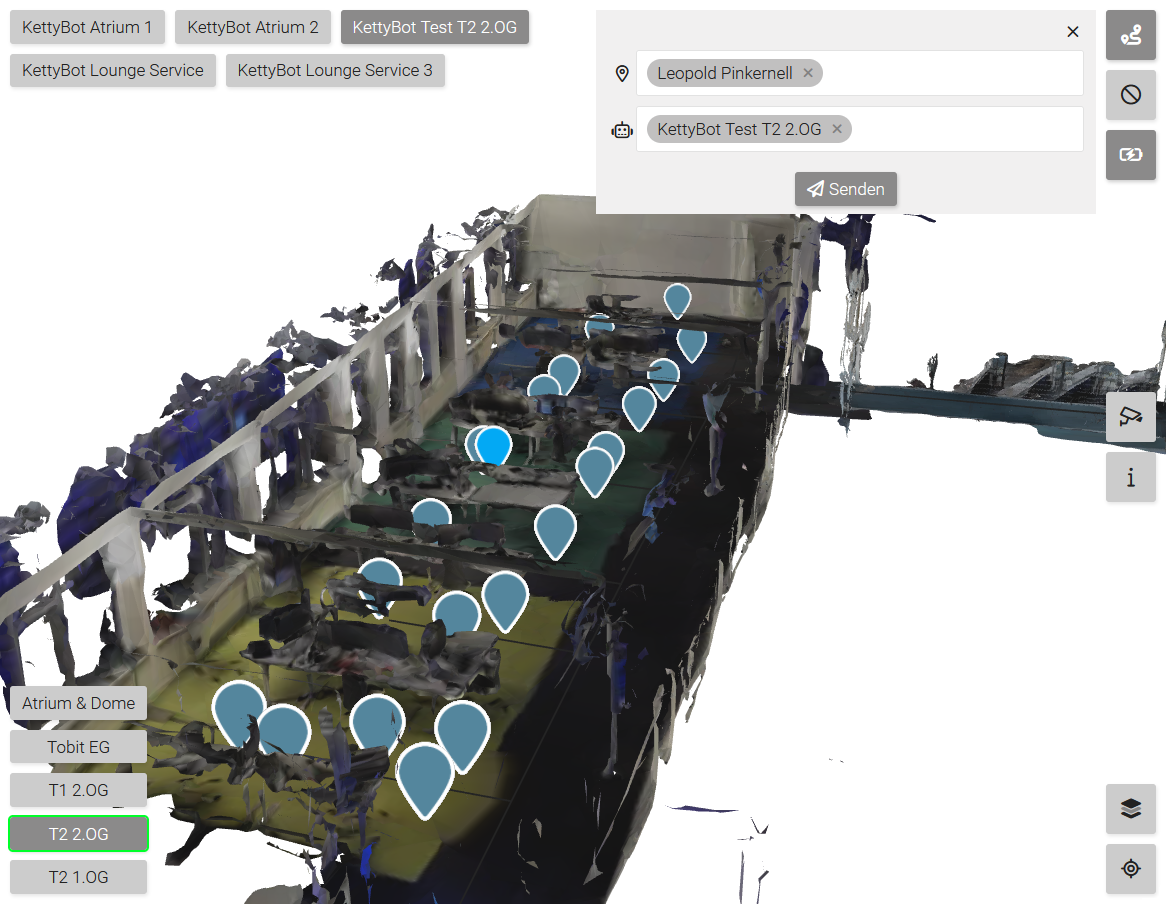
\includegraphics[width=0.9\textwidth]{Screenshot Steuerung.png}
    \\
    Quelle: Eigene Darstellung
\end{figure}

\subsubsection{Verwaltungsansicht}
Die Verwaltungsansicht ist nicht besonder komplex, da die Daten der Roboter und Stockwerke sauber strukturiert sind und somit leicht mithilfe von React gemappt werden können. Hiermit ist gemeint, dass beispielsweise die Liste der Stockwerke leicht mithilfe der map() Funktion in eine Liste an React Komponenten umgewandelt werden kann, die darughin gerendert werden können\cite{ReactMapping}.

In der Roboterliste werden im Gegensatz zum Mockup mehr Statusinformationen der Roboter angezeigt. Auch können mehr Einstellungen der Roboter geändert werden. Da die Übersicht über die verschiedenen Standorte auch über die Liste der Stockwerke ersichtlich ist und dadurch redundant ist, ist diese nicht in der Roboterliste vorhanden. Bei der Abbildung \ref{fig:RobotlistScreenshot} handelt es ich um einen Screenshot der Verwaltung im Prototyp. Man sieht einen geöffneten Roboter-Eintrag, das Kontextmenü, über das Einstellungen geändert werden können und einen Tooltip, in dem eine Statusinformation erläutert wird.

\begin{figure}[H]
    \caption{Verwaltung}\label{fig:RobotlistScreenshot}
    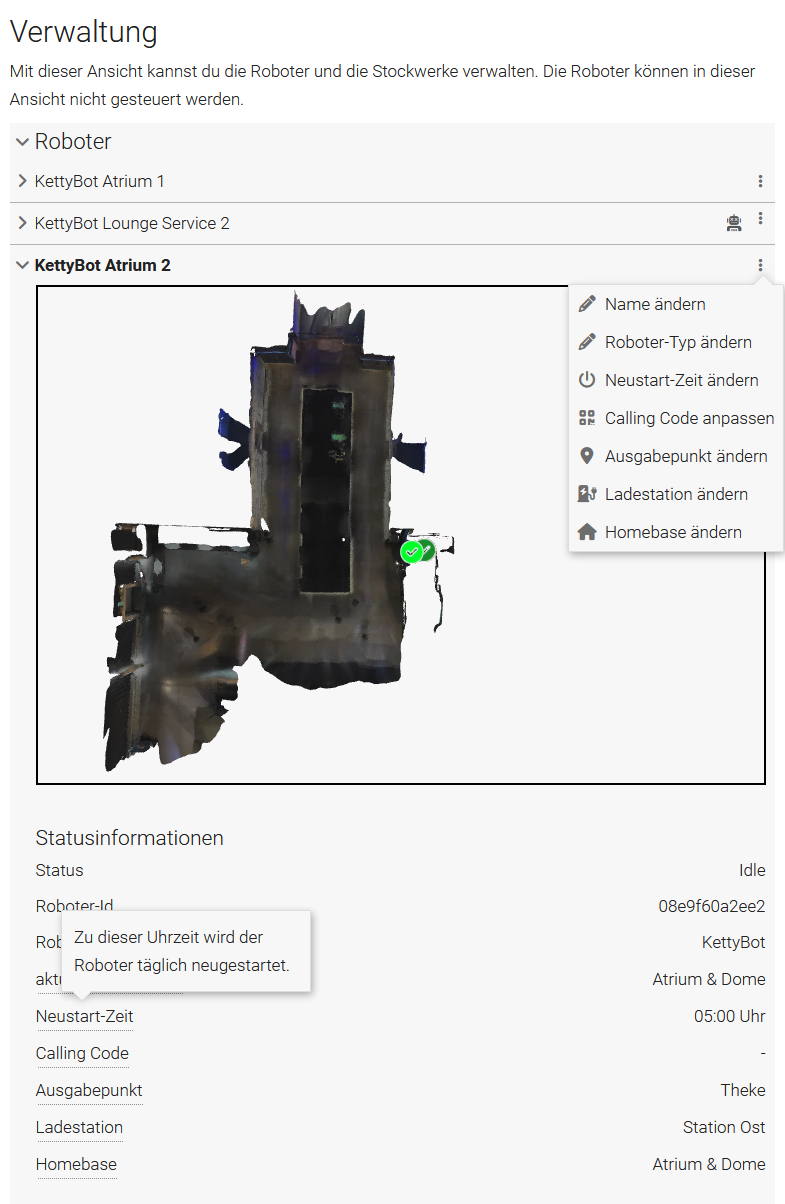
\includegraphics[width=0.6\textwidth]{Screenshot Verwaltung.png}
    \\
    Quelle: Eigene Darstellung
\end{figure}

Die Stockwerkliste unterscheidet sich nur geringfügig vom Mockup. So werden die Standorte im Gegensatz zum Mockup gruppiert nach der Art des Standorts aufgelistet. Der Grund hierfür ist, dass die Art des Standortes nicht unbedingt aus dem Namen ersichtlich. Durch die Gruppierung der Standorte wird eine bessere Übersichtlichkeit über die verschiedenen Standorte erreicht als im Mockup.

In beiden Listen gibt es eine Vorschau des entsprechenden Stockwerks, um die Position des Roboters oder der Standorte zu zeigen. Hierbei handelt es sich um die Nutzeransicht mit reduzierten Funktionen. Die Vorschau ist im Mockup automatisch geöffnet, was ein Problem ist, da die entsprechende \deckgl{}-Karteninstanz - aufgrund des Verhaltens der genutzten Aufklapper-Komponente - beim Öffnen des Aufklappers initialisiert wird. Die Initialisierung der \deckgl{}-Karteninstanz ist rechnerisch aufwändig und verursacht dadurch beim ersten Öffnen des Aufklappers starke Ruckler. Um dieses Verhalten zu verbessern wird stattdessen ein Button angezeigt, über den die Karte manuell initialisiert werden kann. Dadurch gibt es die Ruckler erst beim Klicken des Buttons und nicht beim Öffnen des Aufklappers, was weniger störend ist.

\subsubsection{Editiermodus}
In Verwaltungsansicht, sowie in der Nutzeransicht gibt es die Möglichkeit in den Editiermodus eines Stockwerks zu wechseln. Hier können die Roboterdaten und 3D-Modelle manuell synchronisiert werden. Der Editiermodus ähnelt der Nuteransicht und unterscheidet sich nur durch andere Buttons und die Editiermöglichkeiten. Da der Einsatz der Steuerungs- und Umschalttaste nötig ist, kann dieser Modus nicht an Mobilgeräten genutzt werden. Im Editiermodus hat der Nutzer die Möglichkeit neue 3D-Modelle zu importieren. Hierfür gibt es einen einfachen Dateiinput der nur Dateien im \glb{} Format erlaubt. Wie bereits erwähnt sind die 3D-Modelle im Prototyp hartkodiert. Entsprechend werden Änderungen sowie neu importierte 3D-Modelle nur für die aktuelle Sitzung gespeichert und gehen verloren, wenn die Anwendung erneut geöffnet wird und somit eine neue Sitzung gestartet wird. Mithilfe der in \deckgl{} integrierten Events onDragStart, onDrag und onDragEnd \cite{DeckglInteractivity} kann das angeklickte 3D-Modell per Ziehen der Maus verschoben und rotiert werden. So wird das ausgewählte Modell beim Ziehen entweder verschoben oder rotiert, je nachdem ob die Steuerungs- oder Umschalttaste gedrückt wurden. Das Verschieben und Rotieren kann mithilfe der Tastenkombination Strg + Z rückgängig gemacht und mit Strg + Y wiederholt werden. Hierfür wurden zwei Stapelspeicher implementiert in denen die vergangenen und rückgängiggemachten Aktionen per push hinzugefügt und pop wieder herausgenommen werden. Bei Abbildung \ref{fig:EditmodeScreenshot} handelt es sich um einen Screenshot des Editiermodus. Oben Links gibt es Buttons rückgängigmachen und wiederholen. Mit dem Button oben rechts kann die initiale Kameraposition geändert werden. Unten rechts sind Buttons zum Importieren neuer Modelle, wobei das Importieren nicht impementiert ist, ein Button, über den man die verschiedenen Tastaturshortcuts angezeigt bekommt und einen Button zum Zurücksetzen der Kameraposition. Außerdem gibt es unten Buttons zum Speichern und Abbrechen des Editieren.

\begin{figure}[H]
    \caption{Editiermodus}\label{fig:EditmodeScreenshot}
    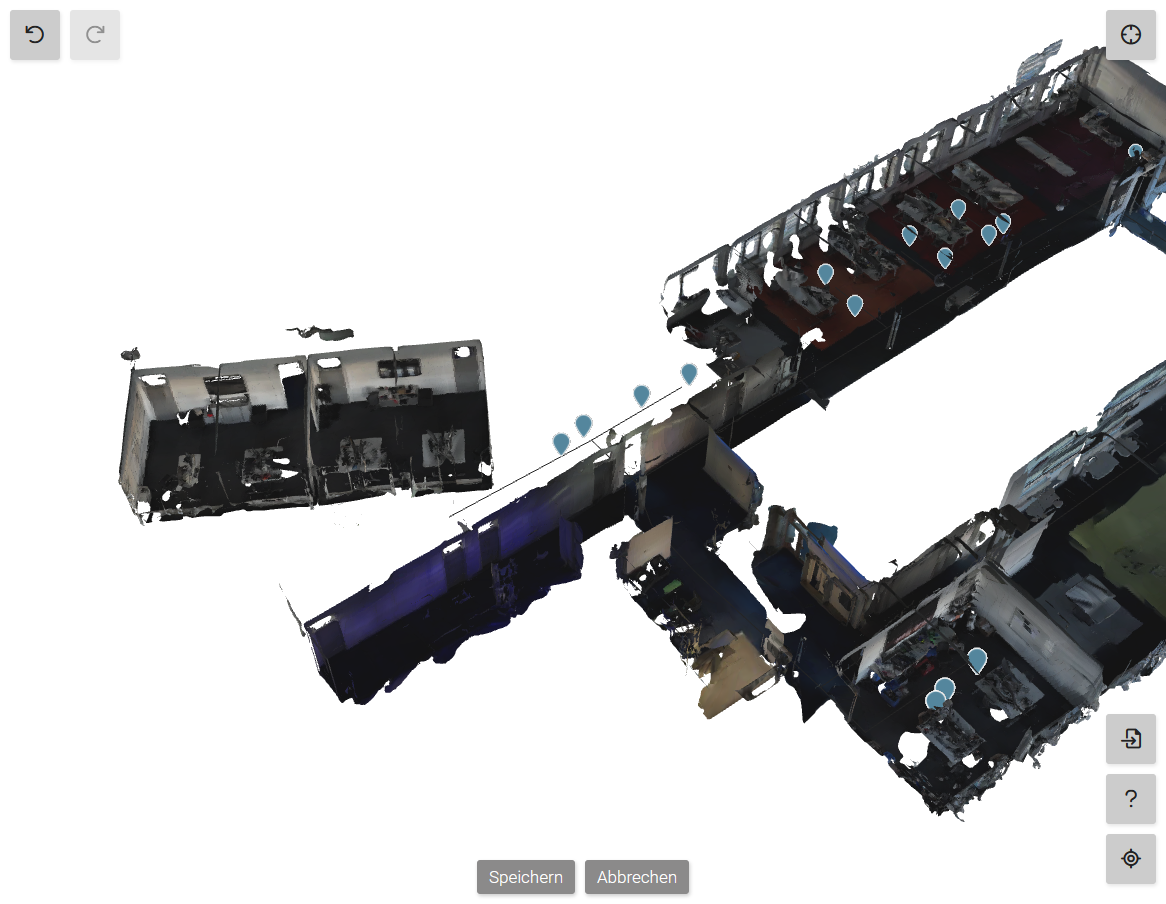
\includegraphics[width=0.9\textwidth]{Screenshot Editiermodus.png}
    \\
    Quelle: Eigene Darstellung
\end{figure}

Der Boden der 3D-Modelle liegt relativ konstant auf der z-Koordinate - der vertikalen Position - 0. Aufgrund der Ungenauigkeiten die durch den \ac{LiDAR}-Scan entstehen ist der Boden aber nicht vollständig eben. Da die Roboterdaten zweidimensional sind und somit keine vertikale Position haben besteht die Gefahr, dass diese an manchen Stellen unter dem Boden der 3D-Modelle verschwinden, wenn sie auf der z-Koordinate 0 angezeigt werden. Aus diesem Grund werden die Roboterdaten an einer leicht erhöhten z-Koordinate positioniert. Da der Boden bei allen 3D-Modellen an derselben z-Koordinate positioniert ist, müssen diese durch den Nutzer nicht weiter an der z-Achse verschoben werden. Im Vergleich zu den Roboterdaten sind die 3D-Modelle immer um 90° an der z-Achse und einen beliebigen Wert an der y-Achse rotiert, während die Rotation der x-Achse zwischen 3D-Modellen und Roboterdaten bereits übereinstimmt. Die 3D-Modelle werden im Editiermodus automatisch um -90° an der z-Achse rotiert und müssen vom Nutzer somit nur nach an der y-Achse rotiert werden können. Die Roboterdaten und 3D-Modelle teilen sich bereits denselben Maßstab, weshalb der Nuter nicht die Möglichkeit braucht die Modelle zu skalieren. Es gilt zu beachten, dass im Prototyp 3D-Modellen aus der Scaniverse App erwartet werden. In einem Produktivsystem sollten auch andere Quellen genutzt werden können. Dort gilt die Annahme dann nicht mehr, dass die Modelle nicht um die z-Koordinate verschoben, nicht um die x- und z-Achse rotiert und nicht skaliert werden müssen. Somit bräuchte der Nutzer in einem Produktivsystem die Möglichkeit Modelle an allen Achsen zu verschieben und um alle Achsen zu rotieren. Auch müsste der Nutzer die Modelle skalieren können.

\subsection{Deployment}

Für das Veröffentlichen des Prototyps wird GitHub Actions in Kombination mit GitHub Pages genutzt. Mit GitHub Actions lassen sich die Build-, Test- und Deploymentpipeline eines Projekts automatisieren \cite{GitHubActions}. So wird bei der Aktualisierung des main Branches automatisch ein Build erstellt und mithilfe der actions-gh-pages Github Action für eine Veröffentlichung auf GitHub Pages bereitgestellt. Das GitHub Repository ist so konfiguriert, dass der erstellte Build automatisch mit GitHub Pages veröffentlicht wird. Bei GitHub Pages handelt es sich um einen Hosting-Dienst für statische Websites, der mit den nötigen Daten aus GitHub Repositories Websites veröffentlichen kann \cite{GitHubPages}.

Die Anwendung verwendet verschiedene Funktionen der chayns-api \cite{ChaynsApi}, wie beispielsweise das Anfordern eines Zugangstokens, ohne den bestimmte Funktionen des Backends nicht aufgerufen werden können.
Aus diesem Grund funktioniert die Anwendung nur, wenn sie - wie in der Dokumentation des create-chayns-app Befehls beschrieben \cite{CreateChaynsApp} - als Custom Page auf einer chayns Seite eingebunden ist. Der Zugriff auf die meisten Funktionen des \ac{BCB}s ist so eingeschränkt, dass diese nur auf bestimmten chayns Seiten aufgerufen werden können, sodass die Steuerungs- und Verwaltungsfunktionen nur auf bestimmten chayns Seiten genutzt werden können.

\subsection{Evaluierung des Prototyps}
Im Folgenden wird gezeigt welche funktionalen Anforderungen und inwieweit die nicht funktionalen Anforderungen Usability und Performance erfüllt werden.

\subsubsection{Funktionale Anforderungen}
Im Kapitel \ref{sec:FunctionalRequirements} sind die funktionalen Anforderungen erläutert, wovon die meisten erfüllt sind, weshalb hier nur die nicht erfüllten Anforderungen erwähnt werden. Bei dem Protyp handelt es sich zwar - wie in den Anforderungen definiert - um eine responsive Webanwendung, sie funktioniert allerdings nicht auf allen Geräten vollständig. So können die für die Gebäudemodelle genutzten \ac{glTF}-Modelle nicht im Safari-Browser angezeigt werden, vermutlich weil diese das \ac{WebP} Bildformat für die Texturen nutzen und dieses noch nicht vollständig von Safari unterstützt wird \cite{CanIUseWebP}. Da es sich hierbei um eine Beschränkung des Safari-Browsers handelt, die in Zukunft von Apple behoben werden sollte und weil alle anderen Funktionen des Prototyps auch im Safari-Browser funktionieren, wurde hierfür kein Workaround entwickelt. Während die Positionsänderungen der Roboter animiert werden, ist das bei den Rotationsänderungen aufgrund eines Bugs in \deckgl{} nicht der Fall. Aus diesem Grund ist die Anforderung, dass der Roboter in der Übersicht fährt nur teilweise erfüllt. Alle anderen funktionalen Anforderungen wie die an die Nutzerrechte und Verwaltungsansicht konnten erfüllt werden.

Die Anforderungen an die Methode zur Gebäudemodell-Generierung konnten weitestgehend erfüllt werden. Für die Methode wird zwar ein iPhone benötigt, dieses besitzt man als Nutzer aber unter umständen bereits. Das Generieren der Modelle erfordert vergleichsweise wenig Aufwand, wobei dieser davon abhängig ist, wie genau das Scannen durchgeführt wird. Insgesamt ist für  das Scannen ist nur wenig Know-How nötig, da es in der Scanniverse App gut erklärt wird. Die entstandenen Modelle müssen komprimiert werden, wofür beispielsweise das im Kapitel \ref{sec:ModelFileFormat} erwähnte Webtool infrage kommt. Ein 3D-Modell könnte in einem Produktivsystem auch mithilfe des \ac{glTF}-Transform Pakets \cite{glTF-Transform} automatisch beim Import in den Editiermodus komprimiert werden. Die Qualität der erzeugten Modelle variiert zum einen dadurch wie gut der Scann durchgeführt wurde und welche Methode zur Komprimierung des Modells genutzt wird. Vergleichsweise geringe Ungenaugkeiten im Modell haben keinen Einfluss auf die Übersichtlichkeit und damit die Hauptfunktion des Modells. 

\subsubsection{Benutzerfreundlichkeit}
Die Benutzerfreundlichkeit wird sowohl anhand der Erfüllung der Usability Entscheidungsregeln als auch durch die Auswertung von Usability-Tests beurteilt.

\paragraph{Usability Heuristics}\label{sec:UsabilityHeuristics}
Die Usability Entscheidungsregeln konnten weitestgehend eingehalten werden. Im Folgenden wird aufgezeigt wie ein paar Entscheidungsregeln konkret eingehalten werden.

Die erste Regel besagt, dass der Nutzer immer innerhalb einer angemssenen Zeispanne durch geeignete Rückmeldungen mitbekommen sollte, was gerade passiert. Diese Regel ist durch verschiedene Features in der Übersicht und Steuerung erfüllt. Zum einen gibt es die Echtzeit-Aktualisierungen des Roboterstandorts und -status über die \gls{Websocket}-Verbindung mit dem \ac{BCB}. Zum anderen werden Statusänderungen auch über die Farben der Buttons signalisiert. Auch gibt es Wait Cursor, um Ladevorgänge anzuzeigen.

% Die zweite Regel erwartet, dass der Nutzer die Sprache der Anwendung versteht und somit beispielsweise möglichst wenig Fachsprache verwendet wird. In der Steuerung und Verwaltung gibt es nur wenig Text, da vor allem Icons eigesetzt werden. In der Verwaltungsansicht werden möglicherweise unklare Begriffe wie Ladestation über Tooltips erklärt. Außerdem werden Einstellungsänderungen über Dialoge erklärt.

Da Benutzer oft versehentlich Aktionen ausführen, gibt es die dritte Regel, die klar gekennzeichnete Abbruchoptionen fordert, damit unerwünschte Aktionen abgebrochen oder rückgängig gemacht werden können. Um die Kamera wieder in die Ausgangsposition zu bringen, wenn diese versehentlich an eine ungewünschte Position bewegt wurde, gibt es in der Übersicht einen entsprechenden Button. In der Steuerung gibt es außerdem einen Button mit dem der aktuelle Lieferauftrag des Roboters abgebrochen werden kann. Auch gibt es sowohl in der Steuerung als auch in der Verwaltung Bestätigungsdialoge mit denen neue Aktionen und Einstellungsänderungen bestätigt werden müssen. Im Editiermodus gibt es die Möglichkeit das Verschieben und Rotieren von Objekten rückgängig zu machen oder zu wiederholen. Auch gibt es im Editiermodus einen Button mit dem das editieren ohne Speichern abgebrochen werden kann. In Abbildung \ref{fig:DialogScreenshot} wird der Bestätigungsdialog gezeigt, der beim Abbrechen der Roboter Aktionen geöffnet wird.

\begin{figure}[H]
    \caption{Bestätigungsdialog}\label{fig:DialogScreenshot}
    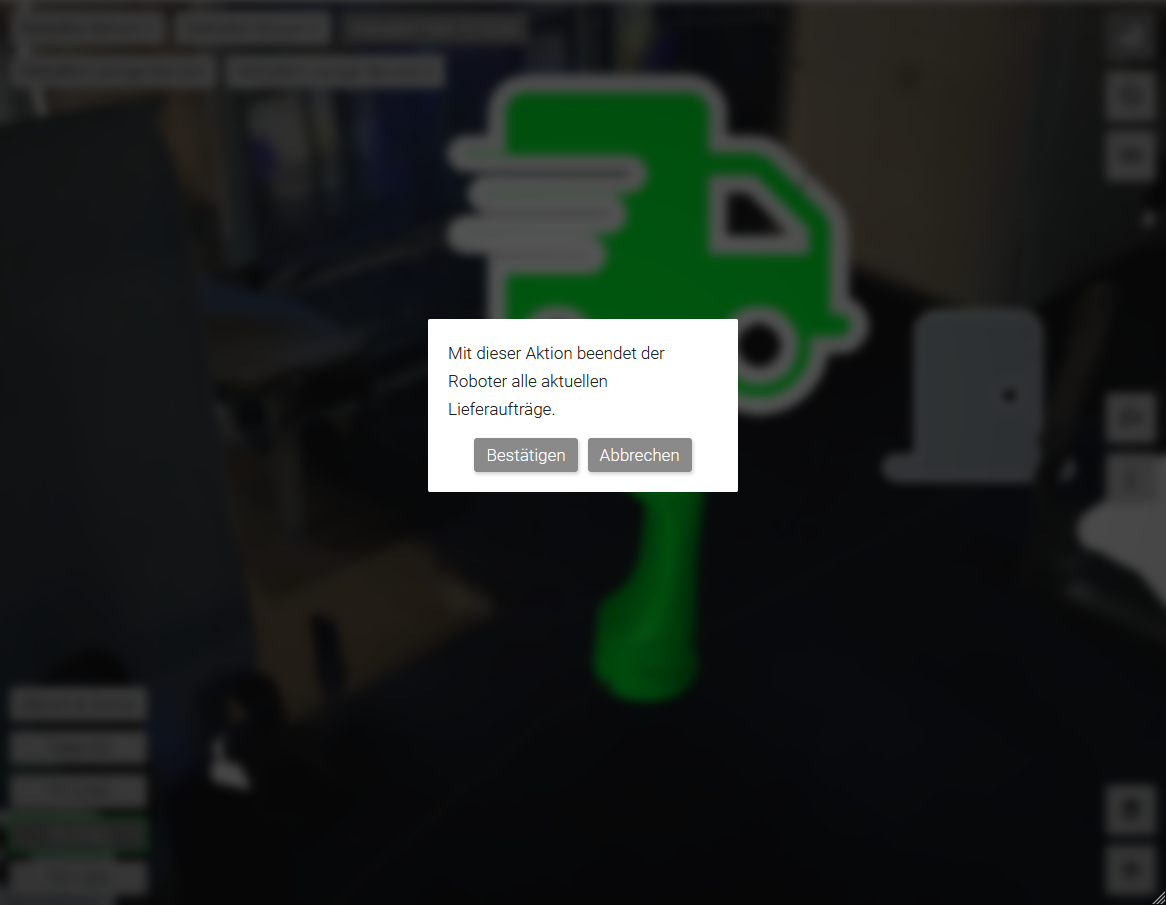
\includegraphics[width=0.9\textwidth]{Screenshot Dialog.png}
    \\
    Quelle: Eigene Darstellung
\end{figure}

% Die vierte Regel sagt aus, dass die UI den Konventionen der Plattform folgen soll und die UI innerhalb der gesamten Anwendung einheitlich ist, damit die Funktion aller Elemente leicht verständlich ist. Diese Regel wird durch den Einsatz der chayns-components für alle GUI Elemente garantiert. So ist die Anwendung sowohl innerlich, als auch unter chayns-Anwendungen einheitlich. 
% TODO ggf. Schaubild in dem Einheitlichkeit zwischen Nutzerkarte und Editiermodus gezeigt wird.
% Die Navigation innerhalb der Karte ist nicht einheitlich mit anderen Kartenanwendungen im Web. So lässt sich die Karte in der Google Maps App mit zwei Fingern vertikal rotieren. Im Prototyp werden stattdessen drei Finger gebraucht. Dieser Umstand ist dem eingesetzten Framework \deckgl{} geschuldet \cite{DeckglController}.

In der fünften Regel geht es darum, dass Probleme, die Fehler auslösen verhindert werden sollten. In der Steuerung ist es zum Beispiel nicht möglich ungültige Standorte in der Routenplanung einzugeben. Währenddessen wird diese Regel in der Verwaltung durch die bereits erwähnten Bestätigungsdialoge erfüllt. Im Editiermodus gibt es die bereits erwähnte Rückgängigmachen und Wiederhohlen Funktion.

% Mit der sechsten Regel wird gefordert, dass sich der Nutzer Informationen zwischen verschiedenen Teilen der Benutzeroberfläche nicht merken muss. Die Anwendung ist so aufgeteilt, dass jeder Nutzer basierend auf seinen Berechtigungen Zugriff auf alle nötigen Informationen hat. In allen Ansichten sind die nötigen Informationen sichtbar, sodass sich Nutzer diese nicht zwischen verschiedenen Ansichten merken müssen.

In der siebten Regel geht darum, dass besimmte häufig genutzte Aktionen mit Shortcuts schneller ausführbar sein sollten. Diese Regel wird in der Steuerung durch die Möglichkeit ermöglicht, den Lieferstandort und Roboter sowohl über die Karte als auch über den Input auswählen zu können. Im Editiermodus gibt es die Shortcuts zum rückgängig machen und wiederhohlen.

% Die achte Regel, die eine minimalistische Benutzeroberfläche erwartet, ist nur subjektiv bewertbar. Mithilfe der Usability Tests kann gut bewertet werden, welche Informationen und Elemente irrelevant sind oder selten gebraucht werden und dadurch überflüssig sind.

% Laut der neunten Regel sollten Fehlermeldungen in einfacher Sparche formuliert sei, das Problem präzise beschreiben und konstruktiv eine Lösung vorschlagen. Hierfür gibt es verschiedene Dialoge die bei Fehlermeldungen angezeigt werden.

% Die zehnte Regel sagt aus, dass es, wenn nötig eine Dokumentation geben sollte, mithilfe welcher die Benutzer ihre Aufgaben verstehen und Abschließen können. Die Anwendung wurde mit dem Ziel entwickelt selbsterklärend zu sein. 
% Dieses Ziel noch irgendwo zu Beginn erwähnen
% Außerdem gibt es Tooltips für bestimmte Statusinformationen und beim Ändern von Einstellungen gibt es Bestätigungsdialoge mit Erklärungen. Mithilfe der Usability Tests kann geprüft werden, ob das Ziel erfüllt werden konnte oder ob weitere Erklärungen nötig sind.

Auch die anderen Usability Entscheidungsregeln wurden während der Entwicklung beachtet und weitestgehend erfüllt, was nicht automatisch bedeutet, dass der Prototyp auch wirklich benutzerfreundlich ist. Um das zu überprüfen, folgen die Usability Tests.

\paragraph{Usability Tests}\label{sec:UsabilityTests}
Während eines Großteils der Implementierung wurden die Usability Tests nur oberflächig durch den Entwickler selbst durchgeführt. Hierdurch wurde während der Entwicklung viel Zeit gespart. So wurde aber auch nur mit einem groben Filter nach Problemen gesucht, sodass viele Probleme nicht identifiziert werden konnten. Aus diesem Grund wurden Usability Tests mit ausgewählten Testpersonen durchgeführt, nachdem alle Funktionen des Prototyps erfolgreich implementiert wurden.

Der Aufbau der ausführlicheren Usability Tests basiert maßgeblich auf verschiedenen Artikeln der Nielsen Norman Group. So wurden die Aufgaben nach dem Stepped-User-Tasks-System \cite{Pernice.2020} formuliert und während der Durchführung der Tests wurde darauf geachtet, dass die Testpersonen die Thinking-Aloud-Methode \cite{Nielsen.2012b} einsetzen. Die ausführlicheren Tests wurden in zwei Runden mit jeweils fünf Personen durchgeführt. So konnten die gefundenen Probleme nach der ersten Runde behoben werden, bevor die zweite Runde durchgeführt wurde. Für die Usability Tests wurden drei Aktivitäten vorbereitet, die die Testpersonen nacheinander durchführen sollten. Die Aktivitäten decken direkt oder indirekt einen großen Teil der Funktionen des Prototyps ab. Konkret beschäftigen sich die Aktivitäten mit der Übersicht, der Steuerung und dem Editiermodus. In der ersten Aktivität müssen Position und Akkustand eines bestimmten Roboters gefunden werden. Daraufhin muss der Roboter in der zweiten Aktivität zu einem oder mehreren Standorten und dann zurück zur Ladestation geschickt werden. In der dritten Aktivität muss ein 3D-Modell mithilfe des Editiermodus richtig positioniert werden. In der dritten Aktivtiät wird beispielsweise nicht nur geprüft wie Benutzerfreundlich das Editieren ist, sondern wie leicht der Editiermodus überhaupt gefunden werden kann.

Um die geplanten Aktivitäten zu prüfen wurde zunächst ein Pilottest durchgeführt.
Mithilfe von Pilottests können Probleme im Design von Tests gefunden werden, sodass diese vor der Durchführung der richtigen Tests aus dem Weg geschafft werden können \cite{Schade.2015}. Mithilfe des Pilottests konnten die Aktivitäten optimiert werden. Außerdem konnten die Ergebnisse des Pilottests bezüglich der Usability des Prototyps ausgewertet werden, sodass viele Probleme behoben werden konnten, bevor die anderen Tests durchgeführt wurden.

\paragraph{Erste Usability Test Runde}

In den beiden folgenden Tabellen werden die Ergebnisse des ersten Usability Test durchlaufs zusammengefasst. Der Pilottest wird hierbei zu dieser Runde dazugezählt und ist in der Tabelle als T0 gekennzeichnet. In Tabelle \ref{tbl:1stUsabilityTestsProblems} wird dargestellt, welche Probleme bei welcher Testperson aufgefallen sind. So sieht man, dass die meisten Probleme die im Pilottest aufgefallen sind, danach nicht mehr aufgetreten sind, was darauf zurückzuführen ist, dass diese vor der Durchführung der restlichen Tests behoben wurden. Man kann zudem sehen, dass den meisten Testpersonen mindestens ein Problem aufgefallen ist, das keiner anderen Testperson aufgefallen ist. Hierdurch zeigt sich, dass durch weniger Testpersonen wahrscheinlich weniger Probleme gefunden worden wären. In Tabelle \ref{tbl:1stUsabilityTestsProblemsDesc} werden die gefundenen Probleme beschrieben. Bei der Korrektur der Probleme wurden die Probleme priorisiert, die besonders vielen Testpersonen aufgefallen sind. Durch die Usability Tests gab es außerdem Feedback von den Testpersonen, welches nicht als Probleme eingestuft wurde, aber trotzdem bei der Implementierung berücksichtigt wurde.

\begin{table}[H]
    \caption{Gefundene Probleme in erster Usability Test Runde}\label{tbl:1stUsabilityTestsProblems}
    \begin{tabular}{l||l|l|l|l|l|l}
                & T0    & T1    & T2    & T3    & T4    & T5    \\ \hline
    Problem 1   & X     &       &       & X     &       &       \\
    Problem 2   & X     &       &       &       &       &       \\
    Problem 3   & X     &       &       &       &       &       \\
    Problem 4   & X     &       &       &       &       &       \\
    Problem 5   & X     &       &       &       &       &       \\
    Problem 6   & X     &       & X     &       &       &       \\
    Problem 7   & X     &       &       &       &       &       \\
    Problem 8   & X     &       &       &       & X     &       \\
    Problem 9   &       & X     &       &       &       &       \\
    Problem 10  &       & X     &       &       &       &       \\
    Problem 11  &       & X     & X     & X     & X     &       \\
    Problem 12  & X     & X     & X     &       &       &       \\
    Problem 13  &       &       & X     &       &       &       \\
    Problem 14  &       &       & X     & X     &       &       \\
    Problem 15  & X     &       & X     &       &       &       \\
    Problem 16  &       &       &       & X     &       &       \\
    Problem 17  &       &       &       & X     &       &       \\
    Problem 18  &       &       &       &       &       & X     \\
    Problem 19  &       &       &       &       &       & X     \\
    Problem 20  &       &       &       &       &       & X     \\
    \end{tabular}    
\end{table}

In Tabelle \ref{tbl:1stUsabilityTestsActions} sind die Aktivitäten in verschiedene Aktionen aufgeteilt, die bei der Ausführung der Aktivität durchgeführt werden können, aber nicht unbedingt durchgeführt werden müssen. Die Werte zeigen, wie gut eine Aktion von einer Testperson durchgeführt werden konnte. Je niedriger der Wert, desto weniger Probleme sind aufgetreten. Kein Wert bedeutet, dass die Testperson die Aktion nicht durchgeführt hat, da die Aktion für den Erfolg der Aktivität nicht benötigt wurde. Somit wird die Usability in den entsprechenden Teilen der Anwendung ersichtlich. Man sieht, dass die meisten Aktionen nach dem Pilottest deutlich besser durchgeführt werden konnten, was auf die erwähnten Anpassungen am Prototyp zurückzuführen ist. Tabelle \ref{tbl:1stUsabilityTestsActions} zeigt, dass die meisten Aktionen zuverlässig durchgeführt werden können, sie zeigt aber auch, dass die Usability an einigen Stellen noch ausbaufähig ist. Insbesondere der Editiermodus hat Mängel, aber auch in der Übersicht und Steuerung gibt es kleinere Probleme.


\begin{table}[H]
    \caption{Bewertung der durchgeführten Aktionen in erster Usability Test Runde}\label{tbl:1stUsabilityTestsActions}
    \begin{tabular}{l||llllll}
        Aktion                              & T0        & T1        & T2        & T3        & T4        & T5        \\ \hline
        \textbf{Aktivität 1 (Übersicht)}    &           &           &           &           &           &           \\
        Roboter mit Button ausgewählt       &         1 &         1 &         1 &         1 &         1 &         1 \\
        Akkustand gefunden                  &         2 &         1 &         1 &         2 &         2 &         1 \\
        Roboter mit Folgen-Button gefunden  &         2 &         1 &         1 &         - &         - &         - \\
        Roboter mit Karte gefunden          &         - &         - &         - &         2 &         1 &         1 \\ \hline

        \textbf{Aktivtiät 2 (Steuerung)}    &           &           &           &           &           &           \\
        Lieferauftrag-Button gefunden       &         1 &         1 &         1 &         1 &         1 &         1 \\
%       Roboter mit Karte ausgewäht         &         - &         - &         - &         - &         - &         1 \\
        Standort mit Personfinder ausgewählt&         2 &         - &         1 &         1 &         1 &         1 \\
        Standort mit Karte ausgewählt       &         - &         1 &         - &         - &         1 &         1 \\
        Lieferauftrag gestartet             &         3 &         2 &         1 &         1 &         1 &         1 \\
        Roboter zur Ladestation geschickt   &         - &         1 &         1 &         1 &         1 &         1 \\ \hline

        \textbf{Aktivität 3 (Editiermodus)} &           &           &           &           &           &           \\
        Editormodus über Adminansicht       &         3 &         - &         - &         - &         - &         - \\
        Editormodus über Nutzeransicht      &         - &         1 &         1 &         1 &         1 &         1 \\
        Steuerung verstanden                &         - &         1 &         3 &         1 &         2 &         1 \\
        Undo/Redo genutzt                   &         - &         - &         - &         - &         - &         - \\
        Modell positioniert                 &         2 &         1 &         2 &         1 &         1 &         1 \\
    \end{tabular}
\end{table}


\paragraph{Zweite Usability Tests Runde}

Die Ergebnisse der ersten Usability Tests Runde wurden in der darauffolgenden Implementierungsphase einbezogen. Verschiedene Probleme wurden behoben und Feedback wurde umgesetzt. Daraufhin wurde eine neue Runde an Usability Tests mit fünf neuen Testpersonen durchgeführt. Die Ergebnisse sind in den folgenden zwei Tabellen abgebildet. Die Tabellen folgen der Struktur der vorherigen Tabellen. So zeigt Tabelle \ref{tbl:2ndUsabilityTestsProblems}, welche Testperson welche Probleme hatte und Tabelle \ref{tbl:2ndUsabilityTestsActions} wie gut Aktionen durchgeführt werden konnten. In Tabelle \ref{tbl:2ndUsabilityTestsProblemsDesc} werden die gefundenen Probleme beschrieben. Man sieht in Tabelle \ref{tbl:2ndUsabilityTestsProblems}, dass deutlich weniger Probleme aufgefallen sind. Neben den Problemen gab es auch noch weiteres Feedback, dass sich aber vor allem auf Rechtschreibung, Zeichensetzung und Benennung beschränkt. Außerdem ist aus dem Feedback erkenntlich, dass das erste Auffinden von bestimmten Funktion etwas dauern kann, die Bedienung dieser Funktionen dann aber einwandfrei funktioniert. Es ist zu erwarten, dass die Bedienung des Prototyps bei einer erneuten Nutzung deutlich leichter ist, da die Funktionen dann nicht mehr lange gesucht werden müssen.

\begin{table}[H]
    \caption{Gefundene Probleme in zweiter Usability Test Runde}\label{tbl:2ndUsabilityTestsProblems}
    \begin{tabular}{l||l|l|l|l|l|l}
                    & T1    & T2    & T3    & T4    & T5    \\ \hline
        % Beim entfernen der Roboter Auswahl wird fälschlicherweise in das Stockwerk des Roboters gewechselt bei dem die Auswahl entfernt wurde
        Problem 1   & X     &       &       &       &       \\
        % Steuerungsbuttons müssen nicht immer aktiv sein (Abbrechen, wenn kein Lieferauftrag existiert; Laden, wenn bereits geladen wird)
        Problem 2   & X     &       &       &       &       \\
        % Roboter kann nicht über die Karte (ohne den "zur Ladestation" Button) zur Ladestation geschickt werden
        Problem 3   &       & X     &       &       &       \\
        % Suchfunktion von Standorten wurde nicht gefunden, weil diese im Lieferauftrag versteckt ist
        Problem 4   &       &       & X     &       &       \\
        % Irritation, dass Erklärung der Steuerung im Tooltip steht und nicht einfach permanent angezeigt an einer anderen Position angezeigt wird
        Problem 5   &       &       &       & X     &       \\
        % Editiermodus im Adminmodus nicht gefunden
        Problem 6   &       &       &       &       & X     \\
        % Editiermodus im Nutzermodus nicht gefunden
        Problem 7   &       &       &       &       & X     \\
    \end{tabular}    
\end{table}

Auch in Tabelle \ref{tbl:2ndUsabilityTestsActions} fällt auf, dass deutlich weniger Probleme aufgetreten sind. So gab es nur bei der zweiten und fünften Testperson geringfügige bis erhebliche Probleme. Bei der zweiten Testperson wurde erst versucht den Roboter direkt über eine Auswahl auf der Karte zur Ladestation zu schicken, während die fünfte Testperson Probleme damit hatte den Editiermodus zu finden, wobei hierfür ohne Erfolg in der Verwaltungsansicht gesucht wurde, bevor der Editiermodus in der Nutzeransicht gefunden wurde. So handelt es sich hier um Probleme die bei einer erneuten Nutzung der Anwendung nicht mehr auftreten würden. Nachdem die Tests ausgewertet wurden, wurde der Prototyp angepasst, sodass die beiden genannten Probleme nicht mehr auftreten sollten. Auch die in \ref{tbl:2ndUsabilityTestsProblems} aufgelisteten Probleme wurden behoben.

\begin{table}[H]
    \caption{Bewertung der durchgeführten Aktionen in zweiter Usability Test Runde}\label{tbl:2ndUsabilityTestsActions}
    \begin{tabular}{l||llllll}
        Aktion                              & T1    & T2    & T3    & T4    & T5    \\ \hline
        \textbf{Aktivität 1 (Übersicht)}    &       &       &       &       &       \\
        Roboter mit Button ausgewählt       & 1     & 1     & 1     & 1     & 1     \\
        Akkustand gefunden                  & 1     & 1     & 1     & 1     & 1     \\
        Roboter mit Folgen-Button gefunden  & -     & -     & -     & -     & -     \\
        Roboter mit Karte gefunden          & 1     & 1     & 1     & 1     & 1     \\ \hline
        \textbf{Aktivtiät - (Steuerung)}    &       &       &       &       &       \\
        Lieferauftrag-Button gefunden       & 1     & -     & -     & -     & 1     \\
%       Roboter mit Karte ausgewäht         & -     & -     & -     & -     & -     \\
        Standort mit Personfinder ausgewählt& 1     & -     & -     & -     & 1     \\
        Standort mit Karte ausgewählt       & -     & 1     & 1     & 1     & -     \\
        Lieferauftrag gestartet             & 1     & 1     & 1     & 1     & 1     \\
        Roboter zur Ladestation geschickt   & 1     & 2     & 1     & 1     & 1     \\ \hline
        \textbf{Aktivität 3 (Editiermodus)} &       &       &       &       &       \\
        Editormodus über Adminansicht       & -     & -     & -     & -     & 3     \\
        Editormodus über Nutzeransicht      & 1     & 1     & 1     & 1     & 2     \\
        Steuerung verstanden                & 1     & 1     & 1     & 1     & 1     \\
        Undo/Redo genutzt                   & -     & -     & 1     & -     & 1     \\
        Modell positioniert                 & 1     & 1     & 1     & 1     & 1     \\
    \end{tabular}
\end{table}

Da die Menge der gefundenen Probleme mit dem zweiten Durchlauf der Tests stark abgenommen hat und da die Aktivitäten fast ohne Probleme durchgeführt wurden, wurde auf einen dritten Testdurchlauf verzichtet. Es ist nicht zu erwarten, dass ein dritter Testdurchlauf bedeutende Erkentnisse liefern würde, da aufgrund der Ergebnisse der vorherigen Tests angenommen werden kann, dass nur noch wenige Probleme bestehen, die auch mit einem erneuten Durchlauf nicht unbedingt gefunden werden können. Es ist wichtig zu beachten, dass mit den Usability Tests nicht alle Funktionen des Prototyps getestet wurden. Stattdessen wurden nur die wichtigsten Funktionen getestet die mit \deckgl{} in Verbindung stehen und somit für die Forschungsfrage dieser Arbeit große relevanz haben. Ob die Liste der Roboter und Stockwerke in der Verwaltungsansicht besonders Benutzerfreundlich ist, ist für diese Arbeit nicht besonders relevant, da diese Liste sehr simpel ist und keine besonderen Technologien nutzt. In Kombination mit der Einhaltung der Usability Entscheidungsregeln ist davon auszugehen, dass das Ziel der Benutzerfreundlichkeit ausreichend erfüllt wurde.

\subsubsection{Performance}
% Metriken kurz erklären
% First Contentful Paint
% Largest Contentfult Paint => Nicht nutzbar, da das Rendern der deck.gl Layers nicht über Events erkannt werden kann
% First Input Delay
% Total Blocking Time
% Erläutern warum die Richtwerte nicht erreicht werden können, die Performance aber trotzdem in Ordnung ist



% => Performance Tests (testen welche Maßnahmen welche Performance Auswirkungen haben)
% Maßnahmen
% Nutzung des .glb Formats statt .obj (beides mit und ohne Kompression)
    % Einfluss auf Ladezeiten (Netzwerk und Rendering)
    % Einfluss auf GPU und CPU Auslastung
% Caching der Robotermodelle
% Caching aller anderen Anfragen (Bis auf Roboter)
% Sehr Kurzzeitiges Caching der Roboter
% Initialisierung der Karten Vorschau über Button statt beim Öffnen des Aufklappers (vielleicht nicht ganz passend?)
